\documentclass[11pt,a4paper]{article}

\usepackage[margin=2.5cm,headheight=15pt]{geometry}
\usepackage[T1]{fontenc}
\usepackage{XCharter}
\usepackage[charter,vvarbb,scaled=1.03]{newtxmath}
\usepackage[scaled=0.96]{inconsolata}
\usepackage{microtype}
\usepackage{listings}
\usepackage{xcolor}
\usepackage{amsmath}
% amssymb and newtxmath both define \Bbbk
\let\Bbbk\relax
\usepackage{amssymb}
\usepackage{booktabs}
\usepackage{tikz}
\usetikzlibrary{arrows.meta,positioning,fit,backgrounds,calc}
\usepackage{titlesec}
\usepackage{fancyhdr}
\usepackage[titles]{tocloft}
\usepackage{enumitem}
\usepackage{parskip}
\usepackage[colorlinks=true,linkcolor=black,citecolor=black,urlcolor=accent,pdfusetitle]{hyperref}
\usepackage{url}

% -- palette ---------------------------------------------------------
\definecolor{accent}{HTML}{0B6E56}
\definecolor{accentdark}{HTML}{064936}
\definecolor{rule}{HTML}{C9C3B4}
\definecolor{codebg}{HTML}{F7F6F2}
\definecolor{outbg}{HTML}{EFEDE6}
\definecolor{comment}{HTML}{5A6B5F}
\definecolor{keyword}{HTML}{4A3480}
\definecolor{strcol}{HTML}{8C4020}

% -- headings --------------------------------------------------------
\titleformat{\section}{\Large\bfseries\color{accentdark}}{\thesection}{0.7em}{}
\titleformat{\subsection}{\large\bfseries\color{accentdark}}{\thesubsection}{0.6em}{}
\titlespacing*{\section}{0pt}{1.9ex plus 0.6ex}{0.9ex}
\titlespacing*{\subsection}{0pt}{1.5ex plus 0.5ex}{0.7ex}

% Parts are typeset by hand: article's \part wants its own page, which is a
% lot of white space for a 19-page document.
\newcommand{\tutpart}[2]{%
  \clearpage
  \phantomsection
  \addcontentsline{toc}{part}{#1 --- #2}%
  \markboth{#1}{}%
  \begingroup
    \color{accentdark}\rule{\linewidth}{1.1pt}\par\vspace{0.7ex}
    {\sffamily\bfseries\large\color{accent} #1}\par\vspace{0.2ex}
    {\Huge\bfseries\color{accentdark} #2}\par\vspace{0.9ex}
    \color{rule}\rule{\linewidth}{0.5pt}
  \endgroup
  \vspace{1.4ex}\par}

% -- running heads ---------------------------------------------------
\pagestyle{fancy}
\fancyhf{}
\renewcommand{\headrulewidth}{0.4pt}
\renewcommand{\headrule}{\color{rule}\hrule height 0.4pt}
% article's \sectionmark uppercases and claims the left slot; we want the part
% on the left and the section on the right, in ordinary case.
\renewcommand{\sectionmark}[1]{\markright{\thesection\quad #1}}
\fancyhead[L]{\footnotesize\sffamily\color{accentdark}\leftmark}
\fancyhead[R]{\footnotesize\sffamily\color{accentdark}\rightmark}
\fancyfoot[C]{\footnotesize\sffamily\color{accentdark}\thepage}
\fancypagestyle{plain}{\fancyhf{}\renewcommand{\headrulewidth}{0pt}%
  \renewcommand{\headrule}{}%
  \fancyfoot[C]{\footnotesize\sffamily\color{accentdark}\thepage}}

% -- contents --------------------------------------------------------
\renewcommand{\cftpartfont}{\sffamily\bfseries\color{accentdark}}
\renewcommand{\cftsecfont}{\normalfont}
\setlength{\cftbeforesecskip}{2pt}
\setlength{\cftbeforepartskip}{10pt}
\renewcommand{\cftpartpagefont}{\bfseries}

% -- listings --------------------------------------------------------
\lstdefinelanguage{Rust}{
  keywords={as,break,const,continue,crate,dyn,else,enum,extern,false,fn,for,
            if,impl,in,let,loop,match,mod,move,mut,pub,ref,return,self,Self,
            static,struct,super,trait,true,type,unsafe,use,where,while},
  keywords=[2]{bool,char,i8,i16,i32,i64,u8,u16,u32,u64,usize,isize,f32,f64,
               str,String,Vec,Option,Result},
  sensitive=true, morecomment=[l]{//}, morecomment=[l]{//!},
  morecomment=[s]{/*}{*/}, morestring=[b]",
}
\lstdefinestyle{base}{
  backgroundcolor=\color{codebg},
  basicstyle=\ttfamily\small,
  commentstyle=\color{comment}\itshape,
  keywordstyle=\color{keyword}\bfseries,
  stringstyle=\color{strcol},
  breaklines=true, showstringspaces=false,
  frame=leftline, rulecolor=\color{accent}, framerule=1.4pt,
  framesep=7pt, xleftmargin=11pt, aboveskip=1.2em, belowskip=1.2em,
  numbers=none,
}
\lstdefinestyle{py}{style=base,language=Python}
\lstdefinestyle{rs}{style=base,language=Rust,keywordstyle=[2]\color{keyword!70}}
\lstdefinestyle{out}{style=base,language={},backgroundcolor=\color{outbg},
  basicstyle=\ttfamily\small\color{black!78},rulecolor=\color{rule},
  framerule=1.4pt}
\lstset{style=base}

% A package name is always a link to where you get it.
\newcommand{\pkg}[1]{\href{https://pypi.org/project/#1/}{\texttt{#1}}}
\newcommand{\crate}[1]{\href{https://crates.io/crates/#1}{\texttt{#1}}}
\newcommand{\repo}[1]{\href{https://github.com/carlok/#1}{\texttt{#1}}}

\title{%
  \vspace{-1.5cm}
  {\color{accent}\rule{\linewidth}{1.2pt}}\\[0.6em]
  \bfseries SAT solving for Python and Rust programmers\\[0.35em]
  {\normalfont\large\color{black!62}
   A tutorial for people who know boolean logic\\
   and have never used a solver}\\[0.5em]
  {\color{rule}\rule{\linewidth}{0.5pt}}}
\author{Carlo Perassi}
\date{\small For \href{https://pypi.org/project/cdclkit/}{cdclkit}~0.1.2 and
      \href{https://pypi.org/project/dratify/}{dratify}~0.1.2}

\begin{document}
\maketitle

\begin{quote}
\small
\textbf{Who this is for.} You can read \texttt{(a and not b) or c} and say
whether it is true for given inputs. You have never used a SAT solver, and you
are not sure why you would. This assumes nothing else.

\textbf{What you will be able to do.} Turn a real problem --- scheduling,
colouring, configuration, puzzle --- into something a solver answers in
milliseconds, and know when the answer can be trusted.

Every code block here was executed, and every output is what it actually
printed.
\end{quote}

\tableofcontents
\newpage

\tutpart{Part I}{The theory you need, and no more}

\section{What a SAT problem is}

A \emph{SAT problem} asks one question:

\begin{quote}
Given a boolean formula, is there any assignment of true/false to its variables
that makes the whole thing true?
\end{quote}

That is it. If yes, the formula is \textbf{satisfiable} (SAT) and the solver
hands you an assignment. If no, it is \textbf{unsatisfiable} (UNSAT).

This sounds like a toy. It is not, for one reason: an enormous number of
practical problems are \emph{disguised} SAT problems. Scheduling, routing,
hardware verification, package dependency resolution, timetabling, puzzle
solving --- all of them reduce to ``find an assignment satisfying these
constraints''. SAT solvers have become good enough that translating your
problem into boolean logic and handing it over often beats writing a bespoke
algorithm.

\section{Why you would install this}
\label{sec:why}

Two different answers, because the two packages are for different jobs. Read
the one that applies to you.

\subsection*{If you write Python: \pkg{cdclkit}}

You reach for this when you have a pile of constraints and need any assignment
satisfying all of them. Concretely:

\begin{itemize}
\item \textbf{Rostering and scheduling.} Six nurses, three shifts, nobody works
      two nights in a row, everyone gets a weekend off a month.
\item \textbf{Configuration.} Which package versions can coexist. Which
      hardware options are mutually compatible.
\item \textbf{Assignment.} Exams to rooms and time slots with no clashes.
      Frequencies to transmitters that must not interfere.
\item \textbf{Puzzles and games.} Sudoku, nonograms, Einstein's zebra ---
      genuinely the same shape of problem as the three above.
\end{itemize}

The alternative is writing a backtracking search yourself. That is slow to
write, and the version you write in an afternoon will be far slower than a
solver that has had thirty years of engineering poured into the same loop.
Encoding to SAT hands that part to someone else.

Two things you get that a hand-written search does not:

\begin{itemize}
\item \textbf{When there is no solution, you learn why.} A minimal
      unsatisfiable subset (Section \ref{sec:mus}) names the handful of
      constraints that actually conflict, rather than reporting
      ``infeasible'' and leaving you to bisect a thousand of them by hand.
\item \textbf{When it says ``no'', you can check it.} That is the whole of
      Section \ref{sec:asymmetry}, and it is unusual --- most tools ask you to
      take ``no solution exists'' on faith.
\end{itemize}

\paragraph{When not to.} If your problem is numeric optimisation --- maximise
profit subject to linear constraints over real numbers --- you want a
linear-programming or MIP solver, not this. If you need raw throughput on
industrial instances with millions of clauses, install \pkg{python-sat}, which
ships kissat and CaDiCaL as binary wheels and will be far faster than anything
here.

\paragraph{So what is actually different?} Less than the previous paragraph
might suggest, and it is worth being precise. \pkg{python-sat} installs just as
easily --- wheels on every platform, one small pure-Python dependency --- so
``no dependencies'' buys you very little on its own. Its Python layer is
perfectly readable too.

One difference is real and checkable: \pkg{python-sat} can \emph{emit} DRUP
proofs (\texttt{with\_proof=True}) and ships \textbf{nothing to check them}. Its
solvers are third-party C and C++ compiled into an extension module, so an
UNSAT answer is something you take on trust unless you fetch a separate C tool.
Here, checking is on by default and the checker is a package you can read.

Whether that matters depends entirely on what you are doing. If you are
searching for a solution, it does not. If you are about to act on ``no solution
exists'', it is the only thing that does.

\subsection*{If you write Rust: the \pkg{dratify} crate}

Narrower, and sharper. You install this when you need to \textbf{verify a
proof of unsatisfiability inside a Rust process}.

That sounds niche until you hit it. Something --- a solver in any language, a
model checker, a build tool --- reported that no solution exists, and you are
about to act on that. Ship the hardware. Declare the configuration impossible.
Sign off the safety argument. The report is a bare assertion from a large
optimised program, and you would like evidence.

Until now your options in Rust were to shell out to \texttt{drat-trim} --- C
you have to compile and invoke as a subprocess --- or to trust the solver. This
crate is a dependency-free alternative that does RUP and RAT properly and runs
in-process.

\paragraph{When not to.} If you want to \emph{solve} from Rust, this is not
that; use an established solver crate. This checks proofs. The distinction is
the point of Section \ref{sec:asymmetry}.

\section{Conjunctive normal form}

Solvers do not accept arbitrary formulas. They accept \textbf{CNF}: an AND of
ORs.

\begin{itemize}
\item A \textbf{literal} is a variable or its negation: $a$, $\lnot a$.
\item A \textbf{clause} is an OR of literals: $(a \lor \lnot b \lor c)$.
\item A \textbf{formula} in CNF is an AND of clauses.
\end{itemize}

\[
(a \lor b) \land (\lnot a \lor b) \land (a \lor \lnot b)
\]

To satisfy the formula you must satisfy \emph{every} clause, and to satisfy a
clause you need \emph{at least one} of its literals true. That is the whole
semantics.

\subsection*{Is CNF a limitation?}

No. Every boolean formula can be converted to CNF, and there is a standard
trick (Tseitin encoding) that does it without the exponential blow-up the naive
conversion would cause. It works by naming subexpressions: introduce a fresh
variable $t$ standing for $(x \land y)$, add clauses forcing
$t \leftrightarrow (x \land y)$, and use $t$ from then on.

You rarely do this by hand. The library does it for you --- Section
\ref{sec:encoder} shows the interface.

\section{DIMACS, the file format}

Everyone in this field exchanges CNF in one plain-text format, and you will see
it constantly.

\begin{lstlisting}[style=out]
p cnf 2 3
 1  2 0
-1  2 0
 1 -2 0
\end{lstlisting}

\begin{itemize}
\item \texttt{p cnf 2 3} --- header: 2 variables, 3 clauses.
\item Variables are numbered from \textbf{1}. A negative number means negation.
\item Each clause is a list of literals terminated by \texttt{0}.
\item Lines starting with \texttt{c} are comments.
\end{itemize}

So the file above is exactly
$(a \lor b) \land (\lnot a \lor b) \land (a \lor \lnot b)$, with $a=1$ and
$b=2$.

\section{The asymmetry that matters}
\label{sec:asymmetry}

Here is the thing that makes this field interesting, and it is worth pausing
on.

\textbf{A ``yes'' answer checks itself.} If the solver says satisfiable and
hands you an assignment, you verify it in linear time: walk the clauses, check
each has a true literal. You do not have to trust the solver at all. You do not
even have to understand it.

\textbf{A ``no'' answer does not.} If the solver says unsatisfiable, what has
it given you? Nothing you can check. It is asserting that \emph{none} of the
$2^n$ assignments works. Re-deriving that yourself means redoing the search.

This is not paranoia. Modern SAT solvers are tens of thousands of lines of
aggressively optimised C, and bugs in them are found regularly --- including in
solvers that have won competitions. If your hardware verification tool reports
``no counterexample exists'', you would like that to mean something.

\section{Proofs of unsatisfiability}

The field's answer is that the solver must \textbf{show its work}.

While searching, a solver learns new clauses that are consequences of the
original formula. If it can eventually derive the \textbf{empty clause} --- a
clause with no literals, which cannot be satisfied by anything --- then the
formula is unsatisfiable. Logging that sequence of derived clauses is a
\textbf{DRAT proof}.

A separate program, a \emph{checker}, replays the log and verifies each step
follows from what came before. The checker is small enough to audit, and shares
no code with the solver.

\subsection*{RUP, informally}

The main proof rule is \textbf{RUP} (reverse unit propagation). To justify a
new clause $C$:

\begin{enumerate}
\item Assume $C$ is false, which forces every literal in it to be false.
\item Propagate: any clause with all-but-one literal false forces its remaining
      literal.
\item If that produces a contradiction, $C$ must have been true. Accept it.
\end{enumerate}

There is a stronger rule, \textbf{RAT}, which permits clauses that are not
strictly implied but preserve satisfiability. It is what the ``A'' in DRAT
stands for. You do not need it to use a solver; you need it if you write a
checker.

\section{What a solver actually does}

You do not need this to use one, but a paragraph helps.

Modern solvers use \textbf{CDCL} --- conflict-driven clause learning. Roughly:
pick an unassigned variable and guess a value; propagate the forced
consequences; if you hit a contradiction, analyse \emph{why} and derive a new
clause that forbids the mistake; backtrack and continue. The learned clauses
accumulate, and each one prunes a chunk of the search space. That learning step
is what separates CDCL from brute force, and it is why solvers handle problems
with millions of variables.

\tutpart{Part II}{One problem, end to end}

Before the details, the whole journey once. Same problem, both languages, and
every file that passes between them printed in full --- they are small enough
to read, which is the point of choosing a small problem.

\section{The timetable}

Three exams: Algebra, Biology, Chemistry. Some students are enrolled in both
Algebra and Biology, some in both Biology and Chemistry, some in both Algebra
and Chemistry. Two exams cannot share a slot if a student sits both.

How many slots do you need?

\begin{center}
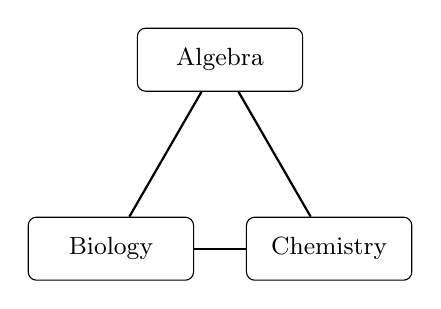
\begin{tikzpicture}[
  node distance=22mm,
  exam/.style={draw, rounded corners=3pt, minimum width=21mm,
               minimum height=8mm, font=\small},
  clash/.style={thick}]
  \node[exam] (A) at (90:16mm) {Algebra};
  \node[exam] (B) at (210:16mm) {Biology};
  \node[exam] (C) at (330:16mm) {Chemistry};
  \draw[clash] (A) -- (B);
  \draw[clash] (B) -- (C);
  \draw[clash] (A) -- (C);
\end{tikzpicture}
\end{center}

An edge means ``shares a student, so cannot share a slot''. Every pair is
joined, so no two exams can be together, so you need three slots. That is
obvious here with three exams. With three hundred it is not, and the useful
part is that the same encoding answers both.

\section{The pipeline}

\begin{center}
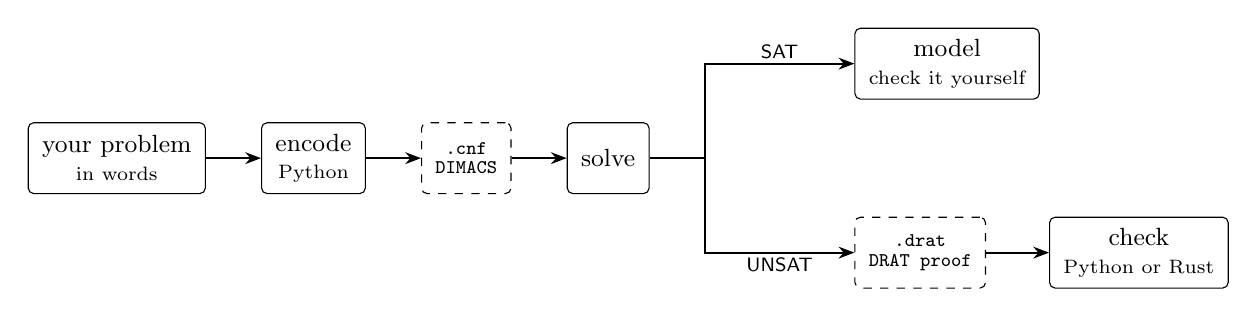
\begin{tikzpicture}[
  box/.style={draw, rounded corners=2pt, align=center, font=\small,
              minimum height=9mm, inner xsep=5pt},
  file/.style={draw, dashed, rounded corners=2pt, align=center,
               font=\ttfamily\scriptsize, minimum height=9mm, inner xsep=5pt},
  arr/.style={-{Stealth[length=2mm]}, thick},
  lbl/.style={font=\scriptsize\sffamily, inner sep=1.5pt, fill=white}]

  \node[box]                      (prob)  {your problem\\[-1pt]\scriptsize in words};
  \node[box,  right=7mm of prob]  (enc)   {encode\\[-1pt]\scriptsize Python};
  \node[file, right=7mm of enc]   (cnf)   {.cnf\\[-1pt]DIMACS};
  \node[box,  right=7mm of cnf]   (solve) {solve};

  % branch targets, placed on two rows so the split is orthogonal
  \node[box,  right=26mm of solve, yshift=12mm]  (model) {model\\[-1pt]\scriptsize check it yourself};
  \node[file, right=26mm of solve, yshift=-12mm] (drat)  {.drat\\[-1pt]DRAT proof};
  \node[box,  right=8mm of drat]                 (check) {check\\[-1pt]\scriptsize Python or Rust};

  \draw[arr] (prob)  -- (enc);
  \draw[arr] (enc)   -- (cnf);
  \draw[arr] (cnf)   -- (solve);

  % right, then up/down, then right again: labels live on the flat runs
  \coordinate (split) at ($(solve.east)+(7mm,0)$);
  \draw[thick] (solve.east) -- (split);
  \draw[arr] (split) |- node[lbl, pos=0.75, above] {SAT}   (model.west);
  \draw[arr] (split) |- node[lbl, pos=0.75, below] {UNSAT} (drat.west);
  \draw[arr] (drat) -- (check);
\end{tikzpicture}
\end{center}

Two exits, and they are not symmetric --- Section \ref{sec:asymmetry} again.
The dashed boxes are plain text files. Nothing in this pipeline is a private
binary format, which is why the Rust half can pick up where the Python half
stopped.

\section{Encoding it}

One boolean per (exam, slot) pair: $x_{e,s}$ is true when exam $e$ sits in slot
$s$. Two kinds of constraint:

\begin{itemize}
\item Every exam gets exactly one slot: \texttt{exactly\_one} over $x_{e,\ast}$.
\item Clashing exams differ: for each clashing pair and each slot,
      $(\lnot x_{a,s} \lor \lnot x_{b,s})$.
\end{itemize}

\lstinputlisting[style=py,firstline=4]{code/ex6_pipeline.py}

\begin{lstlisting}[style=out]
2 slots: UNSAT  (6 vars, 12 clauses)
  proof: 2 additions, 0 deletions
  checked: True
  wrote build/timetable2.cnf and build/timetable2.drat

3 slots: SAT  (9 vars, 21 clauses)
  Algebra    -> slot 3
  Biology    -> slot 2
  Chemistry  -> slot 1
\end{lstlisting}

\section{What actually got produced}

\subsection*{The formula}

Six variables for three exams over two slots. Written out, the whole thing:

\begin{lstlisting}[style=out]
p cnf 6 12
1 2 0        <- Algebra in slot 1 or 2
-1 -2 0      <- ... but not both
3 4 0        <- Biology
-3 -4 0
5 6 0        <- Chemistry
-5 -6 0
-1 -3 0      <- Algebra and Biology not both in slot 1
-2 -4 0      <- ... nor both in slot 2
-3 -5 0      <- Biology and Chemistry
-4 -6 0
-1 -5 0      <- Algebra and Chemistry
-2 -6 0
\end{lstlisting}

Variable $2e+s$ is exam $e$ in slot $s$. The annotations are mine; the file has
none. This is what every SAT tool in the world consumes.

\subsection*{The proof}

\begin{lstlisting}[style=out]
-2 0
0
\end{lstlisting}

Two lines. Read it as: ``Algebra is not in slot 2'' follows from the formula,
and once you have that, the empty clause follows.

Check the first by hand with the RUP rule. Assume the opposite --- Algebra
\emph{is} in slot 2, so variable 2 is true. Then \texttt{-1 -2 0} forces
variable 1 false, and \texttt{1 2 0} is already satisfied. Follow the clashes:
\texttt{-2 -4 0} forces 4 false, so \texttt{3 4 0} forces 3 true; \texttt{-2 -6
0} forces 6 false, so \texttt{5 6 0} forces 5 true. Now 3 and 5 are both true
--- Biology and Chemistry both in slot 1 --- and \texttt{-3 -5 0} forbids
exactly that. Contradiction, so the clause holds.

That is the entire proof system. A checker does this mechanically, for every
line, and reports whether the empty clause is ever reached.

\section{Picking it up from Rust}

The two files are the whole interface. Nothing else passes between the
processes, and the checking side never sees the solver.

\lstinputlisting[style=rs,firstline=4]{code/rust-demo/src/bin/check_files.rs}

\begin{lstlisting}[style=out]
formula: 6 variables, 12 clauses
proof:   2 steps

verified:     true
empty clause: true
by RUP:       2

=> two exam slots really are impossible, and this process
   confirmed it without trusting the solver that said so.
\end{lstlisting}

The parsing is a third of that file, and it is the honest cost of a text
interchange format. What you get for it: the program deciding whether to
believe the answer shares nothing with the program that produced it.

\tutpart{Part III}{Python}

\section{Installing}

\begin{lstlisting}[style=base]
pip install cdclkit            # solver, encodings, modelling layer
pip install "cdclkit[native]"  # the same, plus a Rust engine ~18x faster
\end{lstlisting}

\pkg{cdclkit} depends only on \pkg{dratify}, the proof checker, which has no
dependencies of its own. Nothing third-party is pulled in.

\section{Your first formula}

\lstinputlisting[style=py,firstline=4]{code/ex1_hello.py}

\begin{lstlisting}[style=out]
variables: 2  clauses: 3
satisfiable: True
a = True  b = True
\end{lstlisting}

\texttt{solve} returns a \emph{tuple}. Note the shape --- \texttt{if
solve(f):} is always true, because a two-element tuple is always truthy.
Unpack it.

\section{Unsatisfiable, and proving it}

Forbid all four combinations of two variables and nothing is left.

\lstinputlisting[style=py,firstline=4]{code/ex2_unsat.py}

\begin{lstlisting}[style=out]
satisfiable: False
proof steps: 2 additions, 0 deletions
proof verified by an independent checker: True
empty clause derived: True
\end{lstlisting}

This is Section \ref{sec:asymmetry} made concrete. The solver said ``no'' and
handed over a proof; \pkg{dratify} --- a different package, sharing no solver
code --- replayed it and agreed. You did not have to trust the solver.

\section{Constraints, without writing clauses}
\label{sec:encoder}

Real problems are not phrased as clauses. They are phrased as ``exactly one of
these'', ``at most three of those''. The \texttt{Encoder} turns those into
clauses for you.

\lstinputlisting[style=py,firstline=4]{code/ex3_encoder.py}

\begin{lstlisting}[style=out]
2 colours: UNSAT   (6 vars, 12 clauses)
3 colours: SAT   (9 vars, 21 clauses)
\end{lstlisting}

A triangle needs three colours, and the solver proves two are impossible.

\paragraph{One gotcha.} Internal literals are non-negative --- a variable $v$
is $2v$ positive and $2v{+}1$ negated. So negation is \texttt{neg(x)}, not
\texttt{-x}. This differs from DIMACS on purpose: it makes array indexing
direct in the solver's hot loops. Use \texttt{from\_dimacs} when converting
signed input.

The encoder also offers \texttt{at\_most\_one}, \texttt{at\_least\_k},
\texttt{exactly\_k}, pseudo-boolean constraints
(\texttt{assert\_pb\_leq}), and Tseitin gates (\texttt{and\_gate},
\texttt{or\_gate}, \texttt{xor\_gate}, \texttt{ite}).

\section{The modelling layer}

For most problems you should not touch literals at all. The modelling layer
gives you finite-domain integers.

\lstinputlisting[style=py,firstline=4]{code/ex4_model.py}

\begin{lstlisting}[style=out]
solved: True
    1 3 2 4
    4 2 3 1
    2 4 1 3
    3 1 4 2
\end{lstlisting}

\texttt{int\_var} takes a domain, \texttt{all\_different} does what it says,
and \texttt{cell == 3} builds a constraint. Underneath it is still CNF and
still the same solver --- but you never see a clause.

This is the layer to reach for first. Drop to the encoder when you need a
constraint it does not offer, and to raw clauses almost never.

\section{Why is it unsatisfiable?}
\label{sec:mus}

When a model has no solution, the useful question is which constraints
conflict. A \textbf{minimal unsatisfiable subset} answers it.

\lstinputlisting[style=py,firstline=4]{code/ex5_core.py}

\begin{lstlisting}[style=out]
clause indices in the minimal unsatisfiable subset: [0, 1, 2]
dropping any one of them makes it satisfiable again
\end{lstlisting}

Clause 3 is irrelevant to the contradiction and the MUS excludes it. On a
scheduling problem with a thousand constraints, this is the difference between
``infeasible'' and ``these four requirements cannot all hold''.

\section{The command line}

\begin{lstlisting}[style=base]
cdclkit solve problem.cnf --self-check --check-model
\end{lstlisting}

Solves, and then: if SAT, re-evaluates the model against the original formula
clause by clause; if UNSAT, emits a DRAT proof and has it independently
replayed. Exit codes follow the SAT competition convention --- \texttt{10} for
satisfiable, \texttt{20} for unsatisfiable --- which is unusual enough to
surprise a shell script expecting \texttt{0}.

\tutpart{Part IV}{Rust}

\section{What the Rust crate is for}

The \pkg{dratify} crate is the \emph{proof checker}, not the solver. That is
the piece worth having in Rust: you reach for it when something else produced a
DRAT proof and you need to verify it inside a Rust process, without shelling
out to a C tool.

If you want to \emph{solve} from Rust, use one of the established solvers. If
you want to \emph{check}, this is a dependency-free crate that does RUP and RAT
properly.

\begin{lstlisting}[style=base]
cargo add dratify
\end{lstlisting}

\noindent The crate is \crate{dratify}; the source for both it and the Python
package is \repo{dratify}.

\section{Literals}

The crate uses the same doubled index as the Python side, and getting this
wrong is the most likely first mistake:

\begin{center}
\begin{tabular}{lll}
\toprule
DIMACS & meaning & internal \\
\midrule
\texttt{1}  & $a$       & \texttt{0} \\
\texttt{-1} & $\lnot a$ & \texttt{1} \\
\texttt{2}  & $b$       & \texttt{2} \\
\texttt{-2} & $\lnot b$ & \texttt{3} \\
\bottomrule
\end{tabular}
\end{center}

Variable $v$ becomes $2v$ positive, $2v{+}1$ negated. Negation is a single XOR
with 1, which is why the encoding exists.

\section{Checking a proof}

\lstinputlisting[style=rs,firstline=4]{code/rust-demo/src/main.rs}

\begin{lstlisting}[style=out]
verified:      true
empty clause:  true
steps checked: 2 (2 by RUP, 0 by RAT)

bogus refutation accepted: false
reason: clause is neither RUP nor RAT with respect to the clauses available
        at this point
\end{lstlisting}

The second half matters more than the first. A checker that accepts everything
would pass every test that only feeds it valid proofs. Any checker you rely on
should be tested on proofs that are \emph{wrong}, and should reject them for
the right reason.

\section{What the result tells you}

\texttt{check} returns a \texttt{CheckResult}:

\begin{center}
\begin{tabular}{ll}
\toprule
\texttt{ok} & the proof is a valid refutation \\
\texttt{reached\_empty} & the empty clause was actually derived \\
\texttt{steps}, \texttt{rup\_steps}, \texttt{rat\_steps} & what was checked, and how \\
\texttt{failed\_step}, \texttt{failed\_clause} & where it went wrong, if it did \\
\texttt{reason} & why, in words \\
\bottomrule
\end{tabular}
\end{center}

Note that \texttt{ok} and \texttt{reached\_empty} are separate. A proof whose
every step verifies but which never derives the empty clause is not a
refutation --- it is a valid but incomplete derivation. Conflating the two is
how a truncated proof gets accepted.

\section{Two implementations on purpose}

The Python package ships its own pure-Python checker, and this crate is an
independent implementation of the same rules. Neither is the ``real'' one.

For a proof checker that is the entire point: agreement between independent
implementations is the evidence. They are differentially tested against each
other on rejections as well as acceptances, which is the half that catches a
checker that has quietly started saying yes to everything.

From Python you can have both. \texttt{pip install "cdclkit[native]"} installs
wheels that register the Rust checker with \pkg{dratify}, and
\texttt{check\_proof(..., engine="python")} versus \texttt{engine="native"}
then runs each.

\section*{Where to go next}
\addcontentsline{toc}{section}{Where to go next}

\begin{itemize}[leftmargin=1.3em]
\item \href{https://github.com/carlok/cdclkit/tree/main/examples}%
      {\texttt{examples/}} in the \repo{cdclkit} repository --- Sudoku with a
      uniqueness proof, the zebra puzzle, graph colouring, bounded model
      checking, circuit equivalence.
\item \href{https://github.com/carlok/cdclkit/blob/main/docs/ALGORITHMS.md}%
      {\texttt{docs/ALGORITHMS.md}} --- the mathematics, from resolution
      through first-UIP learning, LBD, DRAT and preprocessing, including a
      section on what is deliberately absent.
\item \href{https://github.com/carlok/cdclkit/blob/main/BENCHMARKS.md}%
      {\texttt{BENCHMARKS.md}} --- how fast this is, and the caveats that
      belong with every number in it.
\item For industrial-scale problems, \pkg{python-sat} bundles kissat and
      CaDiCaL as binary wheels, and is much faster. What it does not do is
      check the proofs it can emit --- see Section \ref{sec:why}.
\item \href{https://github.com/marijnheule/drat-trim}{\texttt{drat-trim}} is
      the reference DRAT checker, in C. \pkg{dratify} agrees with it on every
      proof they have both been given.
\end{itemize}

\end{document}
